% !TEX program = lualatex
% ═══════════════════════════════════════════════════════════════════════
%  Chapitre 4 — Les chaînes de Markov et l'algorithme PageRank
%  Diaporama Beamer pour un exposé magistral (~4 heures)
%  Jérôme Soucy — MAT-2901
%
%  Compilation : lualatex main.tex   (deux passages, pour le sommaire)
%
%  Ce diaporama reprend les définitions, propositions/théorèmes (énoncés
%  seulement), exemples, figures et tableaux du chapitre 4 des notes de
%  cours. Les démonstrations ne sont PAS reproduites : chaque résultat
%  qui, dans les notes, porte une démonstration est plutôt marqué
%  « DÉMONSTRATION AU TABLEAU », avec un rappel très court de l'idée, à
%  l'intention de la personne qui présente.
% ═══════════════════════════════════════════════════════════════════════
\documentclass[aspectratio=169, 11pt]{beamer}
% ═══════════════════════════════════════════════════════════════════════
%  preambule.tex — Réglages, couleurs et raccourcis communs du diaporama
%  du chapitre 4 (« Chaînes de Markov et PageRank »).
%  Ce fichier est autonome : il ne dépend d'aucun fichier du livre.
% ═══════════════════════════════════════════════════════════════════════

% ── Encodage, langue, polices (lualatex, comme le livre) ───────────────
\usepackage{fontspec}
\usepackage[french]{babel}

\setmainfont{TeX Gyre Termes}
\IfFontExistsTF{Fira Sans}
  {\setsansfont{Fira Sans}[Scale=MatchLowercase]}
  {\setsansfont{TeX Gyre Heros}[Scale=MatchLowercase]}
\usefonttheme{professionalfonts}
\renewcommand{\familydefault}{\sfdefault}

\usepackage{amsmath}   % avant unicode-math (sinon \underbrace est cassé)
\usepackage{mathtools}
\usepackage{unicode-math}
\IfFontExistsTF{NewCMMath-Book.otf}
  {\setmathfont{NewCMMath-Book}}
  {\setmathfont{Latin Modern Math}}

\usepackage{booktabs}
\usepackage{array}
\usepackage{graphicx}
\usepackage{adjustbox}
\usepackage{siunitx}
\sisetup{output-decimal-marker = {,}, exponent-product = \times,
         group-separator = {\,}, group-minimum-digits = 4}
\usepackage[skins,breakable]{tcolorbox}
\usepackage{tikz}
\usetikzlibrary{calc, arrows.meta, angles, quotes, patterns, positioning,
                decorations.markings, backgrounds, fit, shapes.geometric}

% ── Palette (identique à celle du livre, livrejs.cls) ──────────────────
\definecolor{sectioncolor}{RGB}{28, 63, 110}   % bleu foncé — titres
\definecolor{thmboxbg}{RGB}{228, 238, 252}     % bleu pâle — énoncés
\definecolor{coveraccent}{RGB}{196, 142, 58}   % or chaud — accent
\definecolor{secboxbg}{RGB}{253, 240, 219}     % ocre pâle — « Pour la classe »
\definecolor{steelblue4}{HTML}{36648B}         % figures : objet de départ
\definecolor{firebrick3}{HTML}{CD3333}         % figures : objet image
\definecolor{demobg}{RGB}{247, 247, 247}       % fond neutre — « au tableau »
\definecolor{bgpage}{RGB}{253, 253, 252}       % fond de diapositive, légèrement chaud

% ── Thème beamer : sobre, cohérent avec le livre ────────────────────────
\usecolortheme{default}
\setbeamercolor{palette primary}{bg=sectioncolor, fg=white}
\setbeamercolor{palette secondary}{bg=sectioncolor, fg=white}
\setbeamercolor{palette tertiary}{bg=sectioncolor, fg=white}
\setbeamercolor{title}{fg=sectioncolor}
\setbeamercolor{frametitle}{bg=sectioncolor, fg=white}
\setbeamercolor{structure}{fg=sectioncolor}
\setbeamercolor{section in toc}{fg=sectioncolor}
\setbeamercolor{subsection in toc}{fg=black}
\setbeamercolor{background canvas}{bg=bgpage}
\setbeamercolor{footline}{fg=gray, bg=bgpage}
\setbeamercolor{block title}{bg=sectioncolor, fg=white}
\setbeamercolor{block body}{bg=thmboxbg, fg=black}
\setbeamercolor{item}{fg=sectioncolor}
\setbeamercolor{itemize item}{fg=coveraccent}
\setbeamercolor{itemize subitem}{fg=sectioncolor}
\setbeamertemplate{itemize item}{\raise0.3ex\hbox{\small$\blacktriangleright$}}
\setbeamertemplate{itemize subitem}{\raise0.3ex\hbox{\footnotesize$\bullet$}}
\setbeamertemplate{navigation symbols}{}
\setbeamerfont{frametitle}{series=\bfseries}
\setbeamertemplate{frametitle}{%
  \vskip-1ex
  \begin{beamercolorbox}[wd=\paperwidth,ht=3.8ex,dp=1.3ex,leftskip=1em,rightskip=1em]{frametitle}
    \bfseries\strut\insertframetitle
  \end{beamercolorbox}
  \vskip3pt
}
\setbeamertemplate{footline}{%
  \leavevmode
  \hbox{\begin{beamercolorbox}[wd=\paperwidth,ht=2.4ex,dp=1ex,leftskip=1em,rightskip=1em]{footline}
    {\scriptsize\color{gray}Chapitre 4 --- Chaînes de Markov et PageRank
    \hfill \insertshorttitle{} \hfill \insertframenumber/\inserttotalframenumber}
  \end{beamercolorbox}}%
}
\setbeamertemplate{blocks}[rounded][shadow=false]
\setbeamertemplate{section in toc}{%
  \inserttocsectionnumber.~\inserttocsection\par\vskip0.15em}

% ── Page de section : diapositive de transition ────────────────────────
\AtBeginSection[]{%
  \begin{frame}[plain,c]
    \begin{center}
      {\color{coveraccent}\rule{0.25\textwidth}{1.2pt}}\\[10pt]
      {\usebeamerfont{frametitle}\usebeamercolor[fg]{title}%
       \Large\bfseries\color{sectioncolor}\insertsectionhead}\\[10pt]
      {\color{sectioncolor}\rule{0.45\textwidth}{0.5pt}}
    \end{center}
  \end{frame}
}
\AtBeginSubsection[]{%
  \begin{frame}[plain,c]
    \begin{center}
      {\large\color{gray}\insertsectionhead}\\[4pt]
      {\Large\bfseries\color{coveraccent}\insertsubsectionhead}
    \end{center}
  \end{frame}
}

% ── Raccourcis mathématiques repris du livre (autonomes) ────────────────
\newcommand{\Plan}{\Pi}
\newcommand{\Transf}{\mathcal{T}}
\newcommand{\Aff}{\mathcal{A}}
\newcommand{\Sim}{\mathcal{S}}
\newcommand{\Iso}{\mathcal{I}}
\newcommand{\mat}[4]{\begin{pmatrix}#1 & #2\\ #3 & #4\end{pmatrix}}
\newcommand{\col}[2]{\begin{pmatrix}#1\\ #2\end{pmatrix}}
\newcommand{\coliii}[3]{\begin{pmatrix}#1\\ #2\\ #3\end{pmatrix}}
\newcommand{\norme}[1]{\lVert #1 \rVert}
\newcommand{\Aire}{\operatorname{Aire}}
\newcommand{\dete}{\operatorname{det}}
\renewcommand{\vec}[1]{\mathbf{#1}}
\DeclareMathOperator{\R}{\mathbb{R}}
\DeclareMathOperator{\Rs}{\mathbb{R}^{\star}}
\newcommand{\intff}[2]{\mathopen{[}{#1},{#2}\mathclose{]}}
\newcommand{\intoo}[2]{\mathopen{]}{#1},{#2}\mathclose{[}}
\newcommand{\defi}[1]{{\color{coveraccent}#1}}
\newcommand{\intfo}[2]{\mathopen{[}{#1},{#2}\mathclose{[}}
\DeclareMathOperator{\N}{\mathbb{N}}
\DeclareMathOperator{\Ns}{\mathbb{N}^{\star}}
\DeclareMathOperator{\Q}{\mathbb{Q}}

% ── Raccourcis propres au chapitre 2 (identiques à macros-livre.tex) ────
\newcommand{\dE}{d_E}                         % distance euclidienne
\newcommand{\dT}{d_T}                         % taxi-distance (Manhattan)
\newcommand{\dHam}{d_{\mathrm{Ham}}}          % distance de Hamming
\newcommand{\dH}{d_H}                         % distance de Hausdorff
\newcommand{\boule}[2]{B(#1, #2)}             % boule ouverte
\newcommand{\Vois}[2]{#1^{\oplus #2}}         % epsilon-voisinage (Minkowski)
\newcommand{\Comp}[1]{\mathcal{K}(#1)}        % compacts non vides de E
\newcommand{\comp}[1]{\mathopen{}#1\mathclose{}^{\mathsf{c}}}

% Images bitmap (portraits, figures Python) reprises du livre.
\graphicspath{{../../figures/portraits/}{../../figures/python/}}

% ── Styles TikZ communs à toutes les figures (identiques au livre) ──────
\tikzset{
  axe/.style        = {-{Stealth[length=2mm]}, gray!70, thin},
  quadrillage/.style= {gray!22, very thin},
  fig/.style        = {fill=steelblue4!22, draw=steelblue4, thick,
                       line join=round},
  figim/.style      = {fill=firebrick3!22, draw=firebrick3, thick,
                       line join=round},
  figaux/.style     = {fill=coveraccent!22, draw=coveraccent!85!black,
                       thick, line join=round},
  pt/.style         = {circle, fill=sectioncolor, inner sep=1.1pt},
  ptim/.style       = {circle, fill=firebrick3, inner sep=1.1pt},
  fleche/.style     = {-{Stealth[length=2.4mm]}, sectioncolor, thick},
  etiq/.style       = {font=\scriptsize, inner sep=1.5pt},
  droite/.style     = {sectioncolor!70, thick, dashed},
}
\newcommand{\repere}[4]{%
  \draw[quadrillage] (#1,#3) grid (#2,#4);
  \draw[axe] (#1,0) -- (#2+0.35,0) node[etiq, below] {$x$};
  \draw[axe] (0,#3) -- (0,#4+0.35) node[etiq, left] {$y$};}
\newcommand{\motifF}{(0,0) -- (0.3,0) -- (0.3,0.55) -- (0.6,0.55) --
  (0.6,0.75) -- (0.3,0.75) -- (0.3,0.85) -- (0.75,0.85) -- (0.75,1) --
  (0,1) -- cycle}

% ── Boîtes d'énoncés (même esprit que le livre : fond bleu pâle) ────────
\tcbset{
  boxenonce/.style={
    enhanced, breakable, colback=thmboxbg, colframe=sectioncolor,
    boxrule=0.6pt, arc=2pt, left=9pt, right=9pt, top=6pt, bottom=6pt,
    fonttitle=\bfseries\sffamily, coltitle=white,
    colbacktitle=sectioncolor, attach boxed title to top left,
    boxed title style={arc=1pt, boxrule=0pt, left=6pt, right=6pt,
      top=3pt, bottom=3pt},
    title style={sharp corners},
  },
  boxclasse/.style={
    enhanced, breakable, colback=secboxbg, colframe=coveraccent,
    boxrule=0.6pt, arc=2pt, left=9pt, right=9pt, top=6pt, bottom=6pt,
    fonttitle=\bfseries\sffamily, coltitle=white,
    colbacktitle=coveraccent, attach boxed title to top left,
    boxed title style={arc=1pt, boxrule=0pt, left=6pt, right=6pt,
      top=3pt, bottom=3pt},
  },
  boxrem/.style={
    enhanced, breakable, colback=white, colframe=steelblue4,
    boxrule=0pt, leftrule=3pt, arc=0pt, left=9pt, right=9pt,
    top=5pt, bottom=5pt,
    colbacktitle=white, coltitle=steelblue4, toptitle=2pt,
    bottomtitle=0pt, fonttitle=\bfseries\sffamily,
  },
  boxoutil/.style={
    enhanced, breakable, colback=white, colframe=steelblue4,
    boxrule=0.6pt, arc=2pt, left=9pt, right=9pt, top=6pt, bottom=6pt,
    fonttitle=\bfseries\sffamily, coltitle=white,
    colbacktitle=steelblue4, attach boxed title to top left,
    boxed title style={arc=1pt, boxrule=0pt, left=6pt, right=6pt,
      top=3pt, bottom=3pt},
  },
  boxtableau/.style={
    enhanced, breakable, colback=demobg, colframe=firebrick3,
    boxrule=0pt, leftrule=4pt, arc=0pt, left=10pt, right=10pt,
    top=7pt, bottom=7pt,
  },
}

% Environnements : titre = « Type N.M — description », fourni en argument.
\newtcolorbox{Enonce}[1]{boxenonce, title={#1}}
\newtcolorbox{Classe}[1]{boxclasse, title={Pour la classe --- #1}}
\newtcolorbox{Outil}[1]{boxoutil, title={Outil --- #1}}
\newtcolorbox{Rem}[1]{boxrem, title={#1}}

% « Démonstration au tableau » : marqueur + rappel très court de l'idée.
\newenvironment{AuTableau}[1][Démonstration au tableau]{%
  \begin{tcolorbox}[boxtableau]
  \bfseries\sffamily\color{firebrick3}\MakeUppercase{#1}\par\nointerlineskip
  \vspace{4pt}\normalfont\rmfamily\upshape\mdseries\color{black}
}{%
  \end{tcolorbox}
}

% Petit renvoi discret vers le numéro du livre, en fin de bloc de titre.
\newcommand{\refnotes}[1]{{\scriptsize\color{gray} (notes de cours, #1)}}

% Insère une figure (tikzpicture ou image) en la contraignant à la fois
% en largeur et en hauteur, sans distorsion : \FigBox[hauteur max]{contenu}.

% ── Raccourcis supplémentaires (identiques à macros-livre.tex / commandesJS.sty)
\newcommand{\dims}{\dim_{\mathrm{sim}}}       % dimension de similitude
\DeclareMathOperator{\eu}{e}
\def\siecle#1{\textsc{\romannumeral #1}\textsuperscript{e}~siècle}
\newcommand{\ap}[1]{\textsuperscript{#1}}
\renewcommand{\P}[1]{\mathbb{P}\mathopen{}\left(#1\right)\mathclose{}}
\newcommand{\Es}[1]{\mathbb{E}\mathopen{}\left(#1\right)\mathclose{}}
\definecolor{vertpiece}{RGB}{58, 125, 68}     % 4e couleur des « pièces »

% Styles TikZ des chapitres 3 et 4 (identiques au livre)
\tikzset{
  fractale/.style   = {fill=sectioncolor},
  nuage/.style      = {fill=sectioncolor},
  courbe/.style     = {sectioncolor, thin, line join=round},
  piece1/.style     = {fill=firebrick3},
  piece2/.style     = {fill=steelblue4},
  piece3/.style     = {fill=coveraccent},
  piece4/.style     = {fill=vertpiece},
  trait1/.style     = {firebrick3, thick, line join=round},
  trait2/.style     = {steelblue4, thick, line join=round},
  trait3/.style     = {coveraccent, thick, line join=round},
  trait4/.style     = {vertpiece, thick, line join=round},
  chaosvers/.style  = {gray!60, dashed, thin},
  chaospas/.style   = {-{Stealth[length=2.2mm]}, firebrick3, thick},
  etat/.style       = {circle, draw=sectioncolor, thick, fill=steelblue4!10,
                       minimum size=9mm, inner sep=1pt, font=\small},
  pageweb/.style    = {etat, minimum size=7.5mm},
  lien/.style       = {-{Stealth[length=2.2mm]}, thick, sectioncolor!85!black},
  lien2/.style      = {{Stealth[length=2.2mm]}-{Stealth[length=2.2mm]}, thick,
                       sectioncolor!85!black},
  proba/.style      = {font=\scriptsize, fill=white, inner sep=1pt},
}

% Les figures du livre chargent leurs données par \input{figures/...} :
% on cherche aussi ces fichiers à la racine du dépôt.
\makeatletter
\def\input@path{{../../}}
\makeatother

% Algorithmes en pseudo-code (même esprit que les boîtes d'énoncés)
\newtcolorbox{Algo}[1]{boxoutil, title={#1}}

% Code Python (sans gras ni italique)
\usepackage{listings}
\lstset{language=Python, basicstyle=\ttfamily\scriptsize,
  keywordstyle=\color{sectioncolor}, commentstyle=\color{gray},
  stringstyle=\color{firebrick3}, columns=fullflexible, keepspaces=true,
  showstringspaces=false, upquote=true, frame=leftline,
  rulecolor=\color{steelblue4}, framerule=2pt, xleftmargin=0pt, framexleftmargin=6pt,
  literate={é}{{\'e}}1 {è}{{\`e}}1 {à}{{\`a}}1 {ç}{{\c c}}1 {ê}{{\^e}}1}

\newcommand{\FigBox}[2][0.56\textheight]{%
  \begin{center}
    \adjustbox{max width=\linewidth, max height=#1}{#2}
  \end{center}}


\title[Chaînes de Markov et PageRank]{Les chaînes de Markov et l'algorithme PageRank}
\subtitle{Chapitre 4 --- MAT-2901 : Mathématiques et technologie}
\author{Jérôme Soucy}
\institute{Université Laval --- Département de mathématiques et de statistique}
\date{}

\begin{document}

\begin{frame}[plain]
  \begin{center}
    {\color{sectioncolor}\rule{0.5\textwidth}{0.8pt}}\\[3pt]
    {\color{coveraccent}\rule{0.14\textwidth}{1.8pt}}

    \vspace{0.55cm}
    {\large\color{gray}Chapitre 4}\\[3pt]
    {\LARGE\bfseries\color{sectioncolor}Les chaînes de Markov\\[2pt]et l'algorithme PageRank}

    \vspace{0.35cm}
    {\normalsize\color{sectioncolor}MAT-2901 --- Mathématiques et technologie}

    \vspace{0.45cm}
    \begin{tikzpicture}[scale=0.42, every node/.style={transform shape}]
      \node[pageweb, fill=sectioncolor!85, text=white] (p1) at (0,2.4) {$1$};
      \node[pageweb, fill=sectioncolor!85, text=white] (p5) at (3.2,2.4) {$5$};
      \node[pageweb, fill=sectioncolor!85, text=white] (p2) at (0,0) {$2$};
      \node[pageweb, fill=sectioncolor!85, text=white] (p3) at (2.2,0) {$3$};
      \node[pageweb, fill=sectioncolor!85, text=white] (p4) at (4.4,0) {$4$};
      \draw[lien2] (p1) -- (p2);
      \draw[lien2] (p2) -- (p3);
      \draw[lien2] (p3) -- (p4);
      \draw[lien] (p3) -- (p5);
      \draw[lien] (p4) -- (p5);
      \draw[lien] (p5) -- (p1);
      \draw[lien] (p5) -- (p2);
    \end{tikzpicture}

    \vspace{0.35cm}
    {\sffamily\color{sectioncolor}Jérôme Soucy}\\[1pt]
    {\small\color{gray}Université Laval}

    \vspace{0.35cm}
    {\color{coveraccent}\rule{0.14\textwidth}{1.8pt}}\\[3pt]
    {\color{sectioncolor}\rule{0.5\textwidth}{0.8pt}}
  \end{center}
\end{frame}

\begin{frame}{Plan de l'exposé}
  \footnotesize
  \begin{columns}[T]
    \begin{column}{0.5\textwidth}
      \tableofcontents[hideallsubsections,sections={1-4}]
    \end{column}
    \begin{column}{0.5\textwidth}
      \tableofcontents[hideallsubsections,sections={5-8}]
    \end{column}
  \end{columns}
\end{frame}

% ═══════════════════════════════════════════════════════════════════════
\section{Un internaute qui navigue au hasard}
% ═══════════════════════════════════════════════════════════════════════

\begin{frame}{Quelles pages sont les plus importantes ?}
  \begin{columns}[c]
    \begin{column}{0.52\textwidth}
      \small
      \begin{itemize}
        \item Une requête : des millions de pages contiennent les mots
          cherchés. Dans quel ordre les présenter ?
        \item Brin et Page (Stanford, fin des années 1990) : imaginons un
          internaute qui clique au hasard sur les liens, et mesurons la
          proportion du temps qu'il passe sur chaque page.
        \item Une page souvent visitée est une page importante : c'est
          l'idée de PageRank, et de Google.
      \end{itemize}
    \end{column}
    \begin{column}{0.46\textwidth}
      \FigBox[0.5\textheight]{%
        \begin{tikzpicture}[scale=1.15]
          \node[pageweb] (p1) at (0,2.4) {$1$};
          \node[pageweb] (p5) at (3.2,2.4) {$5$};
          \node[pageweb] (p2) at (0,0) {$2$};
          \node[pageweb] (p3) at (2.2,0) {$3$};
          \node[pageweb] (p4) at (4.4,0) {$4$};
          \draw[lien2] (p1) -- (p2);
          \draw[lien2] (p2) -- (p3);
          \draw[lien2] (p3) -- (p4);
          \draw[lien] (p3) -- (p5);
          \draw[lien] (p4) -- (p5);
          \draw[lien] (p5) -- (p1);
          \draw[lien] (p5) -- (p2);
        \end{tikzpicture}}
      \scriptsize Figure 4.1 --- Un mini-web de cinq pages. La page $2$
      reçoit quatre liens, la page $1$ deux : où l'internaute
      passera-t-il le plus de temps ?
    \end{column}
  \end{columns}
\end{frame}

\begin{frame}{Une chaîne de Markov}
  \small Le déplacement de l'internaute est une chaîne de Markov : un
  phénomène aléatoire qui évolue par étapes, dont l'état à l'étape $n+1$
  ne dépend que de l'état à l'étape $n$, et non de tout le passé.
  \vspace{4pt}

  Usages : météorologie, démographie, génétique, finance, reconnaissance
  de la parole, génération de texte.
  \vspace{6pt}

  Le chemin du chapitre :
  \begin{enumerate}
    \item rappels de probabilités ;
    \item deux modèles : la météo à deux états, la migration
      ville--banlieue--campagne ;
    \item chaînes de Markov, matrices de transition ;
    \item le long terme : un vecteur propre de valeur propre $1$ ;
    \item PageRank, avec les difficultés du Web réel ;
    \item le calcul par la méthode des puissances --- et le retour du
      théorème de Banach.
  \end{enumerate}
\end{frame}

\begin{frame}{Note historique 4.1 --- Andreï Markov (1856--1922)}
  \footnotesize
  \begin{columns}[T]
    \begin{column}{0.25\textwidth}
      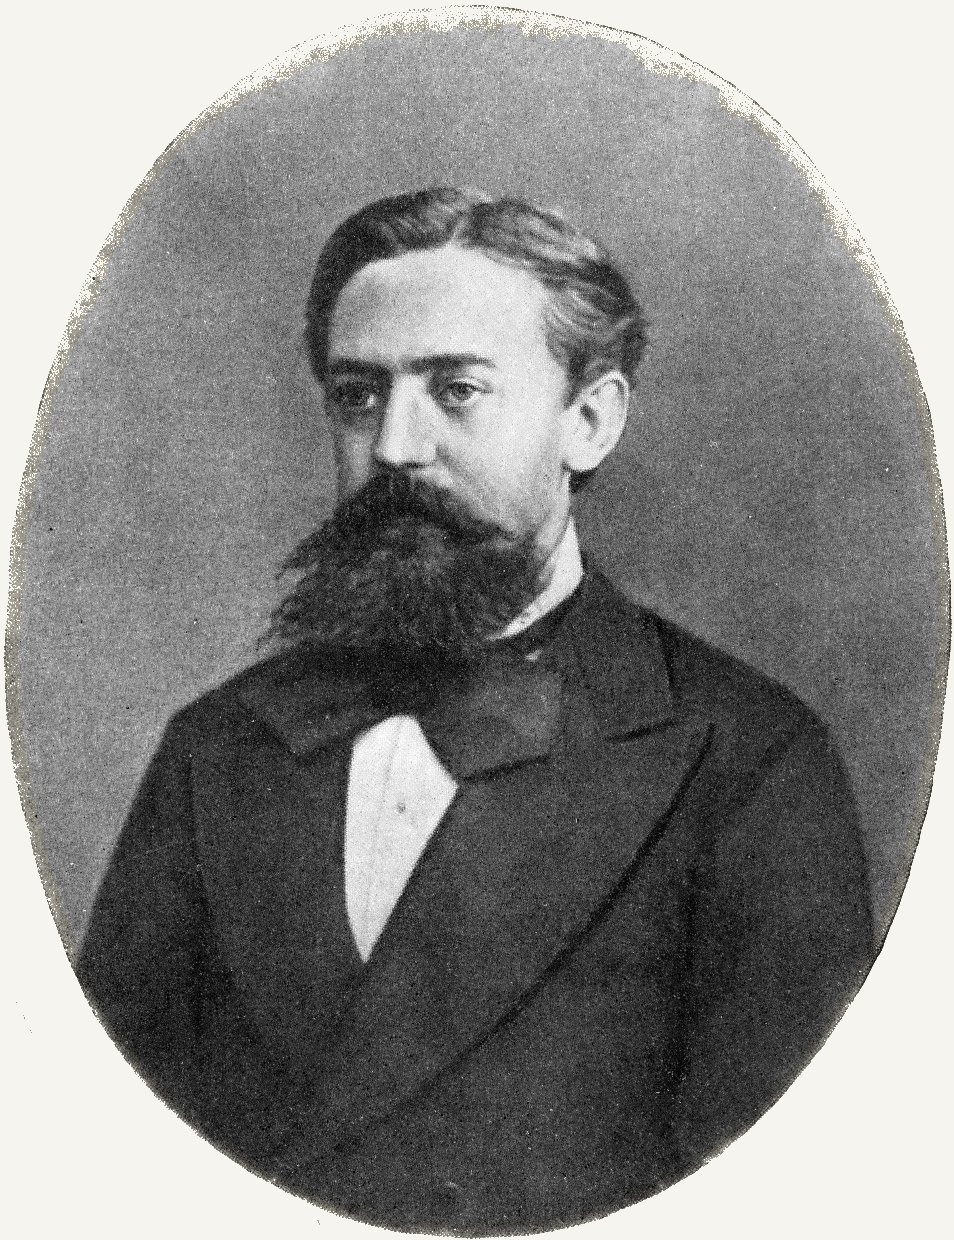
\includegraphics[width=\linewidth]{andrei-markov.jpg}\\
      {\scriptsize\color{gray}Vers 1875. Domaine public,
      Wikimedia Commons.}
    \end{column}
    \begin{column}{0.72\textwidth}
      \begin{itemize}
        \item Né à Riazan ; enfant de santé fragile, il se déplace avec
          des béquilles jusqu'à une dizaine d'années.
        \item Élève de Tchebychev à Saint-Pétersbourg, où il enseigne
          toute sa carrière.
        \item 1906 : ses chaînes, contre Nekrassov, qui soutenait que la
          loi des grands nombres exige l'indépendance (et en tirait des
          conclusions sur le libre arbitre). Markov montre qu'une
          dépendance « au précédent seulement » suffit.
      \end{itemize}
    \end{column}
  \end{columns}
\end{frame}

\begin{frame}{Note historique 4.1 (suite)}
  \small
  \begin{itemize}
    \item Ses chaînes étaient d'abord, pour lui, un contre-exemple
      théorique ; il ne les appliqua qu'une fois à des données réelles
      (note historique 4.2).
    \item Un esprit indépendant : en 1902, il proteste quand l'Académie,
      à la demande du tsar, annule l'élection de Maxime Gorki ; en 1912,
      il demande à être excommunié, par solidarité avec Tolstoï.
    \item En 1913, pendant que l'Empire fête le tricentenaire des
      Romanov, il organise plutôt le bicentenaire de la loi des grands
      nombres (Bernoulli, Ars conjectandi, 1713).
    \item Son fils, Andreï Andreïevitch Markov (1903--1979), sera lui
      aussi mathématicien, spécialiste de logique.
  \end{itemize}
\end{frame}

% ═══════════════════════════════════════════════════════════════════════
\section{Rappels sur les probabilités}
% ═══════════════════════════════════════════════════════════════════════

\begin{frame}{Définition 4.1 --- Probabilité conditionnelle}
  \small Expérience aléatoire, univers (ensemble des résultats),
  événement (sous-ensemble de l'univers), probabilité
  $\P{A}\in\intff{0}{1}$. Une information partielle modifie une
  probabilité : s'il pleut ce matin, l'autobus est plus souvent en
  retard.
  \begin{Enonce}{Définition 4.1 --- Probabilité conditionnelle}
    Soient $A$, $B$ deux événements, avec $\P{B}>0$. La
    \defi{probabilité conditionnelle} de $A$ sachant $B$ est
    \[
      \P{A\mid B} = \frac{\P{A\cap B}}{\P{B}}.
    \]
  \end{Enonce}
  \small Autrement dit $\P{A\cap B}=\P{A\mid B}\,\P{B}$ : la règle
  « multiplier le long d'une branche » d'un diagramme en arbre.
\end{frame}

\begin{frame}{Proposition 4.1 --- Formule des probabilités totales}
  \begin{Enonce}{Proposition 4.1 --- Formule des probabilités totales}
    Soient $B_1,\dots,B_N$ deux à deux incompatibles, de probabilités non
    nulles, de réunion l'univers. Pour tout événement $A$,
    \[
      \P{A} = \P{A\mid B_1}\P{B_1}+\P{A\mid B_2}\P{B_2}+\cdots
      +\P{A\mid B_N}\P{B_N}.
    \]
  \end{Enonce}
  \begin{AuTableau}
    \small Les $A\cap B_j$ sont deux à deux incompatibles, de réunion $A$ ;
    additionner, puis appliquer la définition 4.1.
  \end{AuTableau}
  \small C'est la règle « additionner les branches qui mènent au même
  résultat ».
\end{frame}

\begin{frame}{Exemple 4.1 --- L'autobus du matin}
  \begin{columns}[c]
    \begin{column}{0.5\textwidth}
      \small Il pleut un matin sur trois. S'il pleut, l'autobus est en
      retard avec probabilité $\num{0.4}$ ; sinon, $\num{0.1}$.
      $P$ : « il pleut » ; $R$ : « en retard ».
      \[
        \begin{aligned}
          \P{R} &= \P{R\mid P}\P{P}+\P{R\mid\overline P}\P{\overline P}\\
          &= \num{0.4}\cdot\tfrac13+\num{0.1}\cdot\tfrac23
          = \tfrac{\num{0.6}}{3} = \num{0.2}.
        \end{aligned}
      \]
      L'autobus est en retard un matin sur cinq.
    \end{column}
    \begin{column}{0.48\textwidth}
      \FigBox[0.55\textheight]{%
        \begin{tikzpicture}[grow=right, level distance=2.9cm,
            level 1/.style={sibling distance=2.1cm},
            level 2/.style={sibling distance=1.0cm},
            every node/.style={font=\small},
            edge from parent/.style={draw, sectioncolor!80!black, thick}]
          \node[pt] {}
            child {node[right] {$\overline{P}$}
              child {node[right] {$\overline{R}$ \quad $\tfrac23 \cdot \num{0.9}$}
                     edge from parent node[proba, below] {$\num{0.9}$}}
              child {node[right] {$R$ \quad $\tfrac23 \cdot \num{0.1}$}
                     edge from parent node[proba, above] {$\num{0.1}$}}
              edge from parent node[proba, below] {$\tfrac23$}}
            child {node[right] {$P$}
              child {node[right] {$\overline{R}$ \quad $\tfrac13 \cdot \num{0.6}$}
                     edge from parent node[proba, below] {$\num{0.6}$}}
              child {node[right] {$R$ \quad $\tfrac13 \cdot \num{0.4}$}
                     edge from parent node[proba, above] {$\num{0.4}$}}
              edge from parent node[proba, above] {$\tfrac13$}};
        \end{tikzpicture}}
      \begin{center}\scriptsize Figure 4.2\end{center}
    \end{column}
  \end{columns}
\end{frame}

\begin{frame}{Définition 4.2 --- Variable aléatoire discrète, espérance}
  \begin{Enonce}{Définition 4.2 --- Variable aléatoire discrète}
    \small Une \defi{variable aléatoire discrète} $X$ associe un nombre à
    chaque résultat, et ne prend qu'un nombre fini (ou une suite) de
    valeurs $x_1,x_2,\dots$ Sa \defi{loi} : les $p_i=\P{X=x_i}$, positifs
    et de somme $1$. Son \defi{espérance} :
    $\Es{X} = \sum_i x_i\,p_i$.
  \end{Enonce}
  \small
  \begin{itemize}
    \item Un dé : $\Es{X}=\tfrac16(1+2+\cdots+6)=\num{3.5}$, qui n'est pas
      une valeur possible : c'est une moyenne à long terme.
    \item Linéarité : $\Es{X+Y}=\Es{X}+\Es{Y}$, même sans indépendance.
    \item Indicatrice $\mathbb 1_A$ (vaut $1$ si $A$ se produit, $0$
      sinon) : $\Es{\mathbb 1_A}=\P{A}$.
  \end{itemize}
  Ces deux propriétés permettent de compter en moyenne sans connaître la
  loi d'une somme (exemple 4.2).
\end{frame}

\begin{frame}{Définition 4.3 --- Vecteur de probabilités}
  \small Ici, une variable aléatoire décrit l'état d'un système (le
  temps, un lieu de résidence, une page web), numéroté $1,\dots,N$ : sa
  loi est un vecteur de $\R^N$.
  \begin{Enonce}{Définition 4.3 --- Vecteur de probabilités}
    Un vecteur $\vec p=(p_1,\dots,p_N)$ de $\R^N$ est un \defi{vecteur de
    probabilités} si
    \[
      p_i\geq0 \text{ pour tout } i, \qquad p_1+p_2+\cdots+p_N = 1.
    \]
  \end{Enonce}
  \small
  \begin{itemize}
    \item Dans $\R^2$ : le segment de $(1,0)$ à $(0,1)$ ; dans $\R^3$ : le
      triangle de sommets $(1,0,0)$, $(0,1,0)$, $(0,0,1)$. C'est le
      simplexe de $\R^N$.
    \item Avec $\vec e=(1,1,\dots,1)$ : la condition de somme s'écrit
      $\vec e^{\mathsf T}\vec p=1$.
  \end{itemize}
\end{frame}

\begin{frame}{Pour la classe 4.1 --- Les probabilités conditionnelles au secondaire}
  \begin{Classe}{Les probabilités conditionnelles au secondaire}
    \small
    \begin{itemize}
      \item Diagrammes en arbre dès le primaire ; au deuxième cycle,
        espérance (moyenne pondérée, équité d'un jeu) et décisions à
        partir de probabilités conditionnelles.
      \item L'arbre joue le rôle que jouera la matrice de transition :
        les branches du second niveau portent des probabilités
        conditionnelles, et « multiplier le long d'une branche,
        additionner les branches » est la formule des probabilités
        totales.
      \item Mais un arbre devient vite illisible : avec deux états,
        $2^{10}=1024$ branches après dix étapes. D'où la notation
        matricielle.
    \end{itemize}
  \end{Classe}
\end{frame}

% ═══════════════════════════════════════════════════════════════════════
\section{Un premier modèle : la météo à deux états}
% ═══════════════════════════════════════════════════════════════════════

\begin{frame}{Figure 4.3 --- Le diagramme de transition}
  \small Dans une ville imaginaire :
  \begin{itemize}
    \item après un beau jour : beau le lendemain avec probabilité
      $\num{0.8}$, pluie avec probabilité $\num{0.2}$ ;
    \item après un jour de pluie : beau avec probabilité $\num{0.4}$,
      pluie avec probabilité $\num{0.6}$.
  \end{itemize}
  Seul compte le temps de la veille (ni la saison, ni les jours
  précédents).
  \FigBox[0.3\textheight]{%
    \begin{tikzpicture}
      \node[etat] (B) at (0,0) {$B$};
      \node[etat] (P) at (4,0) {$P$};
      \draw[lien] (B) to[bend left=25] node[proba, above] {$\num{0.2}$} (P);
      \draw[lien] (P) to[bend left=25] node[proba, below] {$\num{0.4}$} (B);
      \draw[lien] (B) to[loop left, min distance=9mm] node[proba, left] {$\num{0.8}$} (B);
      \draw[lien] (P) to[loop right, min distance=9mm] node[proba, right] {$\num{0.6}$} (P);
    \end{tikzpicture}}
  \small Les probabilités des flèches qui partent d'un même état ont une
  somme égale à $1$.
\end{frame}

\begin{frame}{Prévoir le temps des jours suivants}
  \small Il fait beau le jour $0$ ; $X_n$ : le temps dans $n$ jours.
  $\P{X_1=B}=\num{0.8}$. Probabilités totales :
  \[
    \P{X_2=B} = \num{0.8}\cdot\num{0.8}+\num{0.4}\cdot\num{0.2} = \num{0.72}.
  \]
  En général :
  \[
    \left\{\begin{aligned}
      \P{X_{n+1}=B} &= \num{0.8}\,\P{X_n=B}+\num{0.4}\,\P{X_n=P},\\
      \P{X_{n+1}=P} &= \num{0.2}\,\P{X_n=B}+\num{0.6}\,\P{X_n=P}.
    \end{aligned}\right. \tag{4.1}
  \]
  Un produit matriciel : avec $\vec x_n=\big(\P{X_n=B}\,;\ \P{X_n=P}\big)$,
  \[
    \vec x_{n+1} = M\vec x_n,\qquad
    M = \mat{\num{0.8}}{\num{0.4}}{\num{0.2}}{\num{0.6}},\qquad
    \vec x_n = M^n\vec x_0 .
  \]
  $M$ est la matrice de transition ; $m_{ij}$ est la probabilité de
  passer de l'état $j$ à l'état $i$. Prévoir le temps : calculer une
  puissance de matrice.
\end{frame}

\begin{frame}{Remarque 4.1 --- Lignes ou colonnes ?}
  \begin{Rem}{Remarque 4.1}
    \begin{itemize}
      \item Ici, les probabilités qui partent d'un même état forment une
        colonne : $\vec x_{n+1}=M\vec x_n$, comme les vecteurs de
        l'annexe D. La somme de chaque colonne de $M$ vaut $1$.
      \item Beaucoup d'ouvrages de probabilités (et Wikipédia) font
        l'inverse : une ligne, une loi en vecteur ligne $\vec\pi$, et
        $\vec\pi_{n+1}=\vec\pi_nP$.
      \item Équivalent, puisque $P=M^{\mathsf T}$ --- mais il faut repérer
        la convention d'une source avant d'en reprendre les calculs.
    \end{itemize}
  \end{Rem}
\end{frame}

\begin{frame}{Tableau 4.1 --- L'évolution de la loi}
  \small $\P{X_n=B}$, selon le temps du jour $0$ :
  \begin{center}
  \footnotesize
  \begin{tabular}{lcccccccc}
    \toprule
    $n$ & $0$ & $1$ & $2$ & $3$ & $4$ & $5$ & $6$ & $7$ \\
    \midrule
    beau le jour $0$ & $1$ & $\num{0.8}$ & $\num{0.72}$ & $\num{0.688}$ & $\num{0.6752}$ & $\num{0.6701}$ & $\num{0.6680}$ & $\num{0.6672}$ \\
    pluie le jour $0$ & $0$ & $\num{0.4}$ & $\num{0.56}$ & $\num{0.624}$ & $\num{0.6496}$ & $\num{0.6598}$ & $\num{0.6639}$ & $\num{0.6656}$ \\
    \bottomrule
  \end{tabular}
  \end{center}
  \small Dans les deux cas, la loi se rapproche rapidement de
  $\big(\tfrac23\,;\ \tfrac13\big)\approx(\num{0.6667}\,;\ \num{0.3333})$ :
  après une semaine, le temps du jour $0$ n'a presque plus d'influence.
\end{frame}

\begin{frame}{L'état d'équilibre}
  \small Si $\vec x_n\to\vec q$, alors $\vec q=M\vec q$ : un état
  d'équilibre (ou loi stationnaire).
  \begin{itemize}
    \item Algèbre linéaire : un vecteur propre de $M$ associé à la
      valeur propre $1$.
    \item Chapitre 2 : un point fixe de $\vec x\mapsto M\vec x$.
  \end{itemize}
  $(M-I)\vec q=\vec 0$ : $-\num{0.2}\,q_1+\num{0.4}\,q_2=0$ (deux fois),
  d'où $q_1=2q_2$ ; avec $q_1+q_2=1$ :
  \[
    \vec q = \big(\tfrac23\,;\ \tfrac13\big).
  \]
  À long terme, il fait beau deux jours sur trois.
\end{frame}

\begin{frame}{Pourquoi la convergence est-elle si rapide ?}
  \small Polynôme caractéristique :
  $\lambda^2-\num{1.4}\,\lambda+\num{0.4} = (\lambda-1)(\lambda-\num{0.4})$.
  Seconde valeur propre $\lambda_2=\num{0.4}$, vecteur propre
  $\vec v_2=(1,-1)$.
  \vspace{4pt}

  Pour $\vec x_0=(1,0)$ : $\vec x_0=\vec q+\tfrac13\vec v_2$, donc
  \[
    \vec x_n = M^n\vec q+\tfrac13M^n\vec v_2
    = \vec q+\tfrac13(\num{0.4})^n\,\vec v_2 .
  \]
  \begin{itemize}
    \item L'écart à l'équilibre est multiplié par $\num{0.4}$ chaque
      jour : environ $\num{0.0005}$ après une semaine (tableau 4.1).
    \item La seconde valeur propre gouverne la vitesse de convergence
      (on y revient en section 7).
  \end{itemize}
\end{frame}

\begin{frame}{Exemple 4.2 --- Combien de beaux jours dans la semaine ?}
  \small Il fait beau aujourd'hui. $Y$ : le nombre de beaux jours parmi
  les sept suivants. $Y=\mathbb 1_1+\cdots+\mathbb 1_7$, où
  $\mathbb 1_n$ indique « beau le jour $n$ ». Pas d'indépendance, mais la
  linéarité suffit :
  \[
    \Es{Y} = \sum_{n=1}^7\P{X_n=B}
    \approx \num{0.8}+\num{0.72}+\num{0.688}+\cdots+\num{0.6672}
    \approx \num{4.89}.
  \]
  Un peu plus que les $7\cdot\tfrac23\approx\num{4.67}$ jours de
  l'équilibre, puisque la semaine commence par un beau jour.
\end{frame}

\begin{frame}[fragile]{Programme 4.1 --- Le calcul avec Python}
  \begin{columns}[T]
    \begin{column}{0.6\textwidth}
\begin{lstlisting}
import numpy as np
np.set_printoptions(precision=4,
                    suppress=True)

# colonnes : départ d'un beau jour,
#            puis d'un jour de pluie
M = np.array([[0.8, 0.4],
              [0.2, 0.6]])
x0 = np.array([1.0, 0.0])   # il fait beau

for n in [1, 2, 5, 10, 20]:
    print(n, np.linalg.matrix_power(M, n) @ x0)

valeurs, vecteurs = np.linalg.eig(M)
print("valeurs propres :", valeurs)
v = vecteurs[:, np.argmax(valeurs)]  # associé à 1
print("équilibre :", v / v.sum())    # somme = 1
\end{lstlisting}
    \end{column}
    \begin{column}{0.38\textwidth}
      \small
      \begin{itemize}
        \item \texttt{np.linalg.eig} renvoie des vecteurs propres de
          norme $1$ : on divise par la somme des composantes pour obtenir
          un vecteur de probabilités.
        \item Sortie : équilibre $(\num{0.6667}\,;\ \num{0.3333})$,
          valeurs propres $1$ et $\num{0.4}$.
        \item Simulation sur dix mille jours (programme 4.3 des notes) :
          proportion de beaux jours $\num{0.6644}$, proche de $\tfrac23$.
      \end{itemize}
    \end{column}
  \end{columns}
  \vspace{2pt}
  \small Deux lectures de l'équilibre : limite des probabilités, et
  proportion du temps passé dans chaque état --- au cœur de PageRank.
\end{frame}

\begin{frame}{Outil 4.1 --- Puissances de matrices sans programmer}
  \begin{Outil}{Puissances de matrices sans programmer}
    \small
    \begin{itemize}
      \item WolframAlpha : \texttt{\{\{0.8, 0.4\}, \{0.2, 0.6\}\}\^{}10}
        calcule $M^{10}$ ; \texttt{eigenvectors \{\{0.8, 0.4\}, \{0.2,
        0.6\}\}} donne les vecteurs propres.
      \item GeoGebra : \texttt{M = \{\{0.8, 0.4\}, \{0.2, 0.6\}\}}, puis
        \texttt{M\^{}n} avec un curseur $n$ : les deux colonnes de $M^n$
        deviennent presque égales à $\big(\tfrac23\,;\ \tfrac13\big)$.
      \item Si toutes les colonnes de $M^n$ sont proches de $\vec q$, alors
        $M^n\vec x_0$ est proche de $\vec q$ pour tout vecteur de
        probabilités $\vec x_0$ : le point de départ est oublié.
      \item Un tableur convient aussi : une ligne par jour, calculée à
        partir de la précédente par (4.1).
    \end{itemize}
  \end{Outil}
\end{frame}

% ═══════════════════════════════════════════════════════════════════════
\section{Les chaînes de Markov}
% ═══════════════════════════════════════════════════════════════════════

\begin{frame}{Définition 4.4 --- Chaîne de Markov}
  \begin{Enonce}{Définition 4.4 --- Chaîne de Markov}
    \small Une suite de variables aléatoires $X_0,X_1,X_2,\dots$ à
    valeurs dans un ensemble fini d'\defi{états} $\{1,\dots,N\}$ est une
    \defi{chaîne de Markov} si, pour tout $n$ et tous états
    $i,j,i_0,\dots,i_{n-1}$,
    \[
      \P{X_{n+1}=i\mid X_n=j,\ X_{n-1}=i_{n-1},\ \dots,\ X_0=i_0}
      = \P{X_{n+1}=i\mid X_n=j}
    \]
    (\defi{propriété de Markov}). Elle est \defi{homogène} si cette
    probabilité ne dépend pas de $n$ ; on la note $m_{ij}$, et
    $M=(m_{ij})$ est la \defi{matrice de transition}.
  \end{Enonce}
  \small
  \begin{itemize}
    \item Toutes nos chaînes sont homogènes.
    \item Le hasard peut dépendre du passé, mais toute l'information utile
      est contenue dans l'état présent.
    \item Pile ou face : un cas extrême, chaque colonne vaut
      $\big(\tfrac12,\tfrac12\big)$.
  \end{itemize}
\end{frame}

\begin{frame}{Proposition 4.2 --- Évolution de la loi}
  \begin{Enonce}{Proposition 4.2 --- Évolution de la loi}
    Soit $(X_n)$ une chaîne de Markov homogène de matrice $M$, et
    $\vec x_n$ la loi de $X_n$. Alors $\vec x_{n+1}=M\vec x_n$ pour tout
    $n$, et donc $\vec x_n=M^n\vec x_0$.
  \end{Enonce}
  \begin{AuTableau}
    \small Probabilités totales avec $B_j=\{X_n=j\}$ :
    $\P{X_{n+1}=i}=\sum_j m_{ij}\,\P{X_n=j}$, la $i$\ap{e} composante de
    $M\vec x_n$ ; puis récurrence.
  \end{AuTableau}
  \small Avec $\vec x_0=\vec e_j$ : la $j$\ap{e} colonne de $M^n$ est la
  loi de $X_n$ partant de $j$. Le coefficient $(M^n)_{ij}$ est la
  probabilité de passer de $j$ à $i$ en $n$ étapes.
\end{frame}

\begin{frame}{Pour la classe 4.2 --- Graphes et matrices au secondaire}
  \begin{Classe}{Graphes et matrices au secondaire}
    \small
    \begin{itemize}
      \item Le diagramme de transition est un graphe orienté valué :
        sommets = états, arêtes orientées portant un poids.
      \item La progression des apprentissages prévoit une introduction à
        la théorie des graphes au deuxième cycle (graphes orientés et
        valués).
      \item En Technico-sciences, les matrices sont un registre de
        représentation ; on y fait des multiplications matricielles.
      \item Une chaîne de Markov réunit les deux registres : le graphe pour
        décrire, la matrice pour calculer. Passer de l'un à l'autre oblige
        à préciser ce que représente chaque ligne et chaque colonne.
    \end{itemize}
  \end{Classe}
\end{frame}

\subsection{Ville, banlieue et campagne}

\begin{frame}{Figure 4.4 --- Le modèle de migration}
  \small Chaque année : en ville, $\SI{85}{\percent}$ restent,
  $\SI{10}{\percent}$ vont en banlieue, $\SI{5}{\percent}$ à la campagne ;
  en banlieue, $\SI{90}{\percent}$ restent, $\SI{5}{\percent}$ vont en
  ville et $\SI{5}{\percent}$ à la campagne ; à la campagne,
  $\SI{85}{\percent}$ restent, $\SI{10}{\percent}$ vont en banlieue,
  $\SI{5}{\percent}$ en ville. Population constante, taux fixes.
  \FigBox[0.5\textheight]{%
    \begin{tikzpicture}[scale=0.85]
      \node[etat] (V) at (0,0) {$V$};
      \node[etat] (B) at (4,0) {$B$};
      \node[etat] (C) at (2,-3.2) {$C$};
      \draw[lien] (V) to[bend left=15] node[proba] {$\num{0.10}$} (B);
      \draw[lien] (B) to[bend left=15] node[proba] {$\num{0.05}$} (V);
      \draw[lien] (B) to[bend left=15] node[proba] {$\num{0.05}$} (C);
      \draw[lien] (C) to[bend left=15] node[proba] {$\num{0.10}$} (B);
      \draw[lien] (C) to[bend left=15] node[proba] {$\num{0.05}$} (V);
      \draw[lien] (V) to[bend left=15] node[proba] {$\num{0.05}$} (C);
      \draw[lien] (V) to[loop left, min distance=9mm] node[proba, left] {$\num{0.85}$} (V);
      \draw[lien] (B) to[loop right, min distance=9mm] node[proba, right] {$\num{0.90}$} (B);
      \draw[lien] (C) to[loop below, min distance=9mm] node[proba, below] {$\num{0.85}$} (C);
      \node[align=center, anchor=west] at (7.6,-1.4) {%
        $M = \begin{pmatrix}
          \num{0.85} & \num{0.05} & \num{0.05}\\
          \num{0.10} & \num{0.90} & \num{0.10}\\
          \num{0.05} & \num{0.05} & \num{0.85}
        \end{pmatrix}$\\[6pt]
        {\small colonnes : départ de $V$, de $B$, de $C$}\\
        {\small lignes : arrivée en $V$, en $B$, en $C$}};
    \end{tikzpicture}}
\end{frame}

\begin{frame}{Tableau 4.2 --- L'évolution de la répartition}
  \small $\vec x_0=(\num{0.5}\,;\ \num{0.3}\,;\ \num{0.2})$, et
  $\vec x_1=M\vec x_0=(\num{0.45}\,;\ \num{0.34}\,;\ \num{0.21})$.
  \begin{center}
  \footnotesize
  \begin{tabular}{lccccccc}
    \toprule
    $n$ (années) & $0$ & $1$ & $2$ & $5$ & $10$ & $20$ & $50$ \\
    \midrule
    ville & $\num{0.50}$ & $\num{0.45}$ & $\num{0.41}$ & $\num{0.3319}$ & $\num{0.2768}$ & $\num{0.2529}$ & $\num{0.2500}$ \\
    banlieue & $\num{0.30}$ & $\num{0.34}$ & $\num{0.372}$ & $\num{0.4345}$ & $\num{0.4785}$ & $\num{0.4977}$ & $\num{0.5000}$ \\
    campagne & $\num{0.20}$ & $\num{0.21}$ & $\num{0.218}$ & $\num{0.2336}$ & $\num{0.2446}$ & $\num{0.2494}$ & $\num{0.2500}$ \\
    \bottomrule
  \end{tabular}
  \end{center}
  \small Gauss--Jordan sur $M-I$ : le noyau est engendré par $(1,2,1)$,
  d'où $\vec q=\big(\tfrac14,\tfrac12,\tfrac14\big)$. À long terme, la
  moitié de la population vit en banlieue.
\end{frame}

\begin{frame}{Exemple 4.3 --- Une formule exacte pour $\vec x_n$}
  \small Soit $Q=\vec q\,\vec e^{\mathsf T}$ (trois colonnes égales à
  $\vec q$). On vérifie que
  \[
    M = \num{0.8}\,I+\num{0.2}\,Q
  \]
  (première colonne : $(\num{0.8}+\num{0.05}\,;\ \num{0.1}\,;\ \num{0.05})$).
  Chaque année, on garde son lieu avec probabilité $\num{0.8}$ ; avec
  probabilité $\num{0.2}$, on « tire au sort » un milieu selon $\vec q$.
  \begin{itemize}
    \item Si $\vec e^{\mathsf T}\vec v=0$ : $Q\vec v=\vec0$, donc
      $M\vec v=\num{0.8}\,\vec v$ (tout le plan $v_1+v_2+v_3=0$ est
      propre).
    \item $\vec x_0-\vec q$ est dans ce plan, d'où
      \[
        \vec x_n = \vec q+(\num{0.8})^n(\vec x_0-\vec q).
      \]
    \item L'écart diminue de $\SI{20}{\percent}$ par année ;
      $(\num{0.8})^{10}\approx\num{0.107}$. Ce « tirage au sort »
      reviendra dans la matrice Google.
  \end{itemize}
\end{frame}

\subsection{Et si l'avenir dépendait de plusieurs jours ?}

\begin{frame}{Une mémoire de deux jours}
  \begin{columns}[c]
    \begin{column}{0.4\textwidth}
      \begin{center}
      \small
      \begin{tabular}{ccc}
        \toprule
        hier & aujourd'hui & $\P{\text{beau demain}}$ \\
        \midrule
        $B$ & $B$ & $\num{0.9}$ \\
        $P$ & $B$ & $\num{0.7}$ \\
        $B$ & $P$ & $\num{0.5}$ \\
        $P$ & $P$ & $\num{0.3}$ \\
        \bottomrule
      \end{tabular}
      \end{center}
    \end{column}
    \begin{column}{0.58\textwidth}
      \small $(X_n)$ n'est plus une chaîne de Markov. Mais le couple
      $Y_n=(X_{n-1},X_n)$ en est une, à quatre états ($BB$, $PB$, $BP$,
      $PP$) :
      \[
        M_2 = \begin{pmatrix}
          \num{0.9} & \num{0.7} & 0 & 0\\
          0 & 0 & \num{0.5} & \num{0.3}\\
          \num{0.1} & \num{0.3} & 0 & 0\\
          0 & 0 & \num{0.5} & \num{0.7}
        \end{pmatrix}.
      \]
    \end{column}
  \end{columns}
  \small
  \begin{itemize}
    \item Équilibre
      $\vec q=\big(\tfrac{21}{32},\tfrac3{32},\tfrac3{32},\tfrac5{32}\big)$ ;
      beau temps à long terme : $\tfrac{24}{32}=\tfrac34$.
    \item En général, une mémoire de $k$ états donne $N^k$ états. Les
      premiers générateurs de texte : l'état est formé des $k$ derniers
      mots ; plus $k$ est grand, plus le texte est cohérent, mais le
      nombre d'états explose.
  \end{itemize}
\end{frame}

\begin{frame}{Note historique 4.2 --- Les voyelles d'Eugène Onéguine}
  \small En 1913, Markov applique son modèle aux $\num{20000}$ premières
  lettres du roman en vers de Pouchkine, avec deux états : voyelle ou
  consonne.
  \begin{itemize}
    \item $\num{8638}$ voyelles ; une voyelle est suivie d'une voyelle
      $\num{1104}$ fois, soit une fréquence de $\num{0.128}$ ; une
      consonne est suivie d'une voyelle avec une fréquence de
      $\num{0.663}$.
    \item Matrice de transition
      $\mat{\num{0.128}}{\num{0.663}}{\num{0.872}}{\num{0.337}}$.
    \item Équilibre des voyelles :
      $\num{0.663}/(\num{0.872}+\num{0.663})\approx\num{0.432}$,
      exactement la proportion $\num{8638}/\num{20000}$ du texte.
  \end{itemize}
  \vspace{4pt}
  Ce calcul, fait à la main, est la première application d'une chaîne de
  Markov à des données réelles.
\end{frame}

% ═══════════════════════════════════════════════════════════════════════
\section{Matrices stochastiques et états d'équilibre}
% ═══════════════════════════════════════════════════════════════════════

\begin{frame}{Définition 4.5 et proposition 4.3 --- Matrices stochastiques}
  \small Dans les deux modèles, la loi converge vers un unique équilibre,
  quel que soit le départ. Est-ce toujours le cas ?
  \begin{Enonce}{Définition 4.5 --- Matrice stochastique}
    \small Une matrice carrée $M$ est \defi{stochastique} si ses
    coefficients sont positifs ou nuls et si chaque colonne a une somme
    égale à $1$ : chaque colonne est un vecteur de probabilités, et
    $\vec e^{\mathsf T}M=\vec e^{\mathsf T}$.
  \end{Enonce}
  \small Toute matrice de transition est stochastique, et réciproquement.
  \begin{Enonce}{Proposition 4.3 --- Une matrice stochastique conserve les lois}
    \small Si $M$ est stochastique et $\vec v$ un vecteur de probabilités,
    alors $M\vec v$ (et donc $M^n\vec v$) est un vecteur de probabilités.
  \end{Enonce}
  \small Lecture matricielle :
  $\vec e^{\mathsf T}(M\vec v)=(\vec e^{\mathsf T}M)\vec v
  =\vec e^{\mathsf T}\vec v=1$ (le reste : un exercice du chapitre).
\end{frame}

\begin{frame}{Théorèmes 4.4 et 4.5 --- La valeur propre $1$}
  \begin{Enonce}{Théorème 4.4 --- Valeur propre d'une matrice stochastique}
    \small Si $M$ est stochastique, alors $1$ est une valeur propre de $M$.
  \end{Enonce}
  \begin{AuTableau}
    \footnotesize $M$ et $M^{\mathsf T}$ ont le même polynôme
    caractéristique ; et $M^{\mathsf T}\vec e=\vec e$ (transposer
    $\vec e^{\mathsf T}M=\vec e^{\mathsf T}$).
  \end{AuTableau}
  \small Ce vecteur propre a-t-il des composantes positives ?
  Perron--Frobenius (admis) :
  \begin{Enonce}{Théorème 4.5 --- Perron--Frobenius, cas stochastique}
    \small Soit $M$ stochastique. (i) Toute valeur propre $\lambda$
    (réelle ou complexe) vérifie $|\lambda|\leq1$. (ii) Il existe un
    vecteur de probabilités $\vec q$ tel que $M\vec q=\vec q$.
  \end{Enonce}
  \footnotesize Toute chaîne à un nombre fini d'états a au moins un
  équilibre.
\end{frame}

\begin{frame}{Exemples 4.4 et 4.5 --- Deux chaînes qui ne convergent pas}
  \small
  \begin{itemize}
    \item $I$ (taille $2$) : chaque état est conservé. Tout vecteur de
      probabilités est un équilibre, et $\vec x_n=\vec x_0$ : équilibre
      non unique, limite qui dépend du départ. Cela arrive dès que deux
      groupes d'états ne communiquent pas.
    \item $S=\mat{0}{1}{1}{0}$ : l'état change à chaque étape. Unique
      équilibre $\big(\tfrac12,\tfrac12\big)$, mais depuis l'état $1$ la
      loi alterne entre $(1,0)$ et $(0,1)$.
      \begin{itemize}
        \item Valeurs propres $1$ et $-1$ : la composante selon $-1$ change
          de signe au lieu de disparaître. Chaîne périodique.
        \item La proportion du temps passé dans chaque état converge,
          elle, vers $\tfrac12$.
      \end{itemize}
  \end{itemize}
  \vspace{4pt}
  Dans les deux cas, $1$ n'est pas la seule valeur propre de module $1$.
\end{frame}

\begin{frame}{Définition 4.6 --- Matrice stochastique régulière}
  \begin{Enonce}{Définition 4.6 --- Matrice stochastique régulière}
    Une matrice stochastique $M$ est \defi{régulière} s'il existe un
    entier $k\geq1$ tel que tous les coefficients de $M^k$ soient
    strictement positifs.
  \end{Enonce}
  \small
  \begin{itemize}
    \item Après $k$ étapes, tous les états sont accessibles depuis tous
      les états.
    \item Météo et migration : régulières dès $k=1$.
    \item $I$ et $S$ ne le sont pas : leurs puissances valent $I$ ou $S$.
  \end{itemize}
\end{frame}

\begin{frame}{Théorème 4.6 --- Convergence vers l'équilibre}
  \begin{Enonce}{Théorème 4.6 --- Convergence vers l'équilibre}
    \small Soit $M$ une matrice stochastique régulière de taille $N$.
    \begin{enumerate}
      \item[(i)] $1$ est une valeur propre simple de $M$, et toute autre
        valeur propre vérifie $|\lambda|<1$ ;
      \item[(ii)] il existe un unique vecteur de probabilités $\vec q$ tel
        que $M\vec q=\vec q$, à composantes strictement positives ;
      \item[(iii)] pour tout vecteur de probabilités $\vec x_0$,
        $\vec x_n=M^n\vec x_0\to\vec q$.
    \end{enumerate}
  \end{Enonce}
  \begin{AuTableau}
    \footnotesize (i), (ii) : Perron--Frobenius, admis. (iii) si $M$ est
    diagonalisable : $\vec x_0=\alpha_1\vec q+\sum\alpha_i\vec v_i$, donc
    $\vec x_n=\alpha_1\vec q+\sum\alpha_i\lambda_i^n\vec v_i\to\alpha_1\vec q$ ;
    la somme des composantes reste $1$ (prop.~4.3), d'où $\alpha_1=1$.
  \end{AuTableau}
  \small La vitesse : le plus grand $|\lambda_i|$, $i\geq2$. Météo :
  $\num{0.4}$ ; migration : $\num{0.8}$, plus lent (tableaux 4.1 et 4.2).
\end{frame}

\begin{frame}{Remarque 4.2 --- Proportion du temps et temps de retour}
  \begin{Rem}{Remarque 4.2}
    \small
    \begin{itemize}
      \item Première lecture (théorème 4.6) : $\P{X_n=i}\to q_i$.
      \item Deuxième lecture, sur une seule trajectoire : la proportion
        des étapes passées dans l'état $i$ tend vers $q_i$, avec
        probabilité $1$ --- le théorème ergodique (admis), une loi des
        grands nombres pour des étapes dépendantes. Vrai aussi pour les
        chaînes périodiques, si l'équilibre est unique.
      \item Troisième lecture : la chaîne revient en moyenne dans
        l'état $i$ toutes les $1/q_i$ étapes. Météo : un jour de pluie
        tous les $3$ jours, un beau jour tous les $\num{1.5}$ jour.
    \end{itemize}
  \end{Rem}
\end{frame}

\begin{frame}{Pour la classe 4.3 --- Simuler une chaîne de Markov en classe}
  \begin{Classe}{Simuler une chaîne de Markov en classe}
    \small
    \begin{itemize}
      \item Probabilités fréquentielles et théoriques : au cœur de
        l'enseignement dès le premier cycle.
      \item Dé à dix faces : s'il fait beau, « pluie » sur $1$ et $2$ ;
        s'il pleut, « beau » sur $1$ à $4$. Chaque équipe simule un mois ;
        on met en commun.
      \item La proportion de beaux jours se rapproche de $\tfrac23$.
        Question non évidente : pourquoi ne dépend-elle pas du premier
        jour ?
      \item Les jours de pluie arrivent en séquences : l'occasion de
        discuter la conception erronée d'un hasard « bien mélangé ».
    \end{itemize}
  \end{Classe}
\end{frame}

% ═══════════════════════════════════════════════════════════════════════
\section{L'algorithme PageRank}
% ═══════════════════════════════════════════════════════════════════════

\begin{frame}{Contenu et popularité}
  \small Un moteur de recherche classe les pages selon deux types de
  critères :
  \begin{itemize}
    \item le contenu : présence des mots cherchés, position dans le titre
      ou le texte, proximité ;
    \item la popularité, mesurée par la structure des liens du Web.
  \end{itemize}
  PageRank (Brin et Page, 1998) relève du second type.
  \vspace{6pt}

  L'internaute aléatoire : sur une page qui contient $k$ liens, il clique
  sur l'un d'eux, chacun avec probabilité $1/k$. La proportion du temps
  qu'il passe sur une page mesure son importance.
\end{frame}

\subsection{L'internaute aléatoire}

\begin{frame}{La matrice de transition du mini-web}
  \begin{columns}[c]
    \begin{column}{0.55\textwidth}
      \small Départ sur la page $3$ (trois liens : vers $2$, $4$, $5$).
      Pour être sur la page $1$ après deux clics, il faut passer par $2$
      ou par $5$ :
      \[
        \P{X_2=1} = \tfrac12\cdot\tfrac13+\tfrac12\cdot\tfrac13 = \tfrac13.
      \]
      La page visitée est une chaîne de Markov ; $a_{ij}=1/k_j$ si la page
      $j$ (avec $k_j$ liens) pointe vers $i$, $0$ sinon :
      \[
        A = \begin{pmatrix}
          0 & \tfrac12 & 0 & 0 & \tfrac12\\[2pt]
          1 & 0 & \tfrac13 & 0 & \tfrac12\\[2pt]
          0 & \tfrac12 & 0 & \tfrac12 & 0\\[2pt]
          0 & 0 & \tfrac13 & 0 & 0\\[2pt]
          0 & 0 & \tfrac13 & \tfrac12 & 0
        \end{pmatrix}.
      \]
    \end{column}
    \begin{column}{0.43\textwidth}
      \FigBox[0.4\textheight]{%
        \begin{tikzpicture}[scale=1.15]
          \node[pageweb] (p1) at (0,2.4) {$1$};
          \node[pageweb] (p5) at (3.2,2.4) {$5$};
          \node[pageweb] (p2) at (0,0) {$2$};
          \node[pageweb] (p3) at (2.2,0) {$3$};
          \node[pageweb] (p4) at (4.4,0) {$4$};
          \draw[lien2] (p1) -- (p2);
          \draw[lien2] (p2) -- (p3);
          \draw[lien2] (p3) -- (p4);
          \draw[lien] (p3) -- (p5);
          \draw[lien] (p4) -- (p5);
          \draw[lien] (p5) -- (p1);
          \draw[lien] (p5) -- (p2);
        \end{tikzpicture}}
      \small Colonnes : liens qui sortent d'une page. Lignes : liens qui
      y entrent.
    \end{column}
  \end{columns}
\end{frame}

\begin{frame}[fragile]{Programme 4.5 --- Le PageRank du mini-web}
  \begin{columns}[T]
    \begin{column}{0.62\textwidth}
\begin{lstlisting}
def matrice_transition(liens, N):
    """liens[j] : pages vers lesquelles pointe j."""
    A = np.zeros((N, N))
    for j, sorties in liens.items():
        for i in sorties:
            A[i - 1, j - 1] = 1 / len(sorties)
    return A

liens = {1: [2], 2: [1, 3], 3: [2, 4, 5],
         4: [3, 5], 5: [1, 2]}
A = matrice_transition(liens, 5)
valeurs, vecteurs = np.linalg.eig(A)
k = np.argmin(abs(valeurs - 1))
q = np.real(vecteurs[:, k])
q = q / q.sum()
print("fois 55 :", 55 * q)  # [13. 20. 12. 4. 6.]
\end{lstlisting}
    \end{column}
    \begin{column}{0.36\textwidth}
      \small
      \begin{itemize}
        \item \texttt{eig} peut renvoyer des complexes (matrice non
          symétrique) : \texttt{np.real}.
        \item On ne sait pas où se trouve la valeur propre $1$ dans la
          liste : on cherche la plus proche.
        \item Avec $\vec p_0=(0,0,1,0,0)$ :\\
          $\vec p_1=\big(0,\tfrac13,0,\tfrac13,\tfrac13\big)$,\\
          $\vec p_2=\big(\tfrac13,\tfrac16,\tfrac13,0,\tfrac16\big)$.
      \end{itemize}
    \end{column}
  \end{columns}
\end{frame}

\begin{frame}{Le PageRank du mini-web}
  \small
  \[
    \vec q = \tfrac1{55}\,(13, 20, 12, 4, 6).
  \]
  \begin{itemize}
    \item $A$ est régulière (coefficients de $A^5$ tous $>0$) : le
      théorème 4.6 s'applique, quel que soit le départ.
    \item Classement : page $2$, page $1$, page $3$, page $5$, page $4$.
  \end{itemize}
  La deuxième ligne de $\vec q=A\vec q$ :
  \[
    q_2 = 1\cdot q_1+\tfrac13\,q_3+\tfrac12\,q_5
    = \tfrac{13}{55}+\tfrac13\cdot\tfrac{12}{55}+\tfrac12\cdot\tfrac6{55}
    = \tfrac{20}{55}.
  \]
  \begin{itemize}
    \item L'importance d'une page est la somme des « votes » des pages qui
      pointent vers elle ; chaque page partage son PageRank également
      entre ses liens sortants.
    \item La page $1$ (deux liens entrants) devance la page $3$ (deux
      aussi) : l'un de ses liens vient de la page $2$, la plus importante.
    \item Circulaire en apparence ; l'algèbre linéaire en fait la solution
      d'un système.
  \end{itemize}
\end{frame}

\begin{frame}{Note historique 4.3 --- Le gogol et un vecteur propre à 25 milliards}
  \small
  \begin{itemize}
    \item Le projet de Page et Brin sur les liens du Web donne naissance à
      Google (article de 1998).
    \item Google vient de googol (gogol en français) : le nombre
      $10^{100}$. Selon Edward Kasner (Mathematics and the Imagination,
      1940), le mot aurait été inventé par son neveu de neuf ans, Milton
      Sirotta.
    \item Kurt Bryan et Tanya Leise ont popularisé l'analyse mathématique
      de l'algorithme sous le titre « The \$25,000,000,000 eigenvector ».
      Tout repose sur les notions de ce chapitre.
  \end{itemize}
\end{frame}

\subsection{Les pages sans liens sortants}

\begin{frame}{Figure 4.5 --- Le mini-web 2}
  \begin{columns}[c]
    \begin{column}{0.4\textwidth}
      \FigBox[0.55\textheight]{%
        \begin{tikzpicture}[scale=1.05]
          \node[pageweb] (p1) at (0,2.4) {$1$};
          \node[pageweb] (p5) at (3.2,2.4) {$5$};
          \node[pageweb] (p2) at (0,0) {$2$};
          \node[pageweb] (p3) at (2.2,0) {$3$};
          \node[pageweb] (p4) at (4.4,0) {$4$};
          \node[pageweb, fill=firebrick3!15, draw=firebrick3] (p6) at (3.2,4.4) {$6$};
          \draw[lien2] (p1) -- (p2);
          \draw[lien2] (p2) -- (p3);
          \draw[lien2] (p3) -- (p4);
          \draw[lien] (p3) -- (p5);
          \draw[lien] (p4) -- (p5);
          \draw[lien] (p5) -- (p1);
          \draw[lien] (p5) -- (p2);
          \draw[lien] (p5) -- (p6);
        \end{tikzpicture}}
    \end{column}
    \begin{column}{0.58\textwidth}
      \small PDF, images, pages en construction : la page $6$ n'a aucun
      lien. La sixième colonne de $A$ est nulle : $A$ n'est plus
      stochastique, la probabilité « s'échappe ».
      \vspace{4pt}

      Correction : depuis une page sans lien, l'internaute choisit une
      page au hasard parmi les $N$ (probabilité $1/N$ chacune). Avec
      $\vec E$, l'indicatrice des pages sans lien
      ($\vec E=(0,0,0,0,0,1)$ ici) :
      \[
        B = A+\frac1N\,\vec e\,\vec E^{\mathsf T}. \tag{4.2}
      \]
    \end{column}
  \end{columns}
\end{frame}

\begin{frame}{Le PageRank du mini-web 2}
  \small
  \[
    B = \begin{pmatrix}
      0 & \tfrac12 & 0 & 0 & \tfrac13 & \tfrac16\\[2pt]
      1 & 0 & \tfrac13 & 0 & \tfrac13 & \tfrac16\\[2pt]
      0 & \tfrac12 & 0 & \tfrac12 & 0 & \tfrac16\\[2pt]
      0 & 0 & \tfrac13 & 0 & 0 & \tfrac16\\[2pt]
      0 & 0 & \tfrac13 & \tfrac12 & 0 & \tfrac16\\[2pt]
      0 & 0 & 0 & 0 & \tfrac13 & \tfrac16
    \end{pmatrix}
    \qquad \text{stochastique et régulière.}
  \]
  \[
    \vec q = \tfrac1{127}\,(27, 42, 27, 10, 15, 6)
    \approx (\num{0.213}\,;\ \num{0.331}\,;\ \num{0.213}\,;\
    \num{0.079}\,;\ \num{0.118}\,;\ \num{0.047}).
  \]
  Classement : page $2$, pages $1$ et $3$ à égalité, page $5$, page $4$,
  page $6$. Peu de changements : la page $1$ rejoint la page $3$, en
  partie parce que la page $5$ partage maintenant son vote entre trois
  liens.
\end{frame}

\subsection{Les régions piégeantes et la téléportation}

\begin{frame}{Figure 4.6 --- Le mini-web 3 : une région piégeante}
  \begin{columns}[c]
    \begin{column}{0.4\textwidth}
      \FigBox[0.55\textheight]{%
        \begin{tikzpicture}[scale=1.05]
          \node[pageweb] (p1) at (0,2.4) {$1$};
          \node[pageweb] (p5) at (3.2,2.4) {$5$};
          \node[pageweb] (p2) at (0,0) {$2$};
          \node[pageweb] (p3) at (2.2,0) {$3$};
          \node[pageweb] (p4) at (4.4,0) {$4$};
          \node[pageweb, fill=firebrick3!15, draw=firebrick3] (p6) at (3.2,4.4) {$6$};
          \node[pageweb, fill=firebrick3!15, draw=firebrick3] (p7) at (0.8,4.4) {$7$};
          \draw[lien2] (p1) -- (p2);
          \draw[lien2] (p2) -- (p3);
          \draw[lien2] (p3) -- (p4);
          \draw[lien] (p3) -- (p5);
          \draw[lien] (p4) -- (p5);
          \draw[lien] (p5) -- (p1);
          \draw[lien] (p5) -- (p2);
          \draw[lien] (p5) -- (p6);
          \draw[lien2] (p6) -- (p7);
        \end{tikzpicture}}
    \end{column}
    \begin{column}{0.58\textwidth}
      \small Une page $7$, et des liens $6\leftrightarrow7$. On entre dans
      la région $\{6,7\}$ par la page $5$, mais on ne peut plus en sortir.
      \begin{itemize}
        \item $A$ est stochastique mais pas régulière.
        \item Unique équilibre
          $\vec q=\big(0,0,0,0,0,\tfrac12,\tfrac12\big)$ : les pages $1$ à
          $5$ ont un PageRank nul. Inutilisable.
        \item La loi ne converge même pas (aller-retour entre $6$ et $7$,
          comme l'exemple 4.5) ; $-1$ est valeur propre de $A$.
        \item Sur le Web réel, de telles régions se forment spontanément,
          ou délibérément pour accaparer le PageRank.
      \end{itemize}
    \end{column}
  \end{columns}
\end{frame}

\begin{frame}{La téléportation}
  \small À chaque étape, l'internaute suit un lien avec probabilité
  $\beta$, et avec probabilité $1-\beta$ saute vers une page choisie au
  hasard parmi les $N$ (il tape une nouvelle adresse). $\beta\in\intoo01$
  est le facteur d'amortissement ; Brin et Page utilisaient
  $\beta=\num{0.85}$.
  \[
    G = \beta B+(1-\beta)\,U,\qquad U = \frac1N\,\vec e\,\vec e^{\mathsf T}
    \quad\text{(tous les coefficients valent $1/N$).} \tag{4.3}
  \]
  C'est le « tirage au sort » de l'exemple 4.3, avec la loi uniforme.
  \begin{Enonce}{Proposition 4.7 --- Propriétés de la matrice $G$}
    \small Si $0<\beta<1$, $G$ est stochastique à coefficients
    strictement positifs ; elle est donc régulière, et a un unique
    équilibre $\vec q$, à composantes strictement positives.
  \end{Enonce}
  \begin{AuTableau}
    \footnotesize Somme d'une colonne : $\beta\cdot1+(1-\beta)\cdot1=1$ ;
    chaque coefficient est au moins $(1-\beta)/N>0$ ; $k=1$.
  \end{AuTableau}
\end{frame}

\begin{frame}[fragile]{Programme 4.7 --- La matrice Google}
  \begin{columns}[T]
    \begin{column}{0.6\textwidth}
\begin{lstlisting}
def matrice_google(liens, N, beta=0.85):
    A = matrice_transition(liens, N)
    E = (A.sum(axis=0) == 0).astype(float)
    e = np.ones(N)
    B = A + np.outer(e, E) / N    # pages sans sortie
    U = np.outer(e, e) / N        # téléportation
    return beta * B + (1 - beta) * U

def equilibre(M):
    valeurs, vecteurs = np.linalg.eig(M)
    k = np.argmin(abs(valeurs - 1))
    q = np.real(vecteurs[:, k])
    return q / q.sum()

liens3 = {1: [2], 2: [1, 3], 3: [2, 4, 5],
          4: [3, 5], 5: [1, 2, 6],
          6: [7], 7: [6]}
G3 = matrice_google(liens3, 7)
print(equilibre(G3))
\end{lstlisting}
    \end{column}
    \begin{column}{0.38\textwidth}
      \small
      \begin{itemize}
        \item \texttt{np.outer(u, v)} : le produit
          $\vec u\,\vec v^{\mathsf T}$.
        \item \texttt{beta=1} : seulement la correction des pages sans
          lien (mini-web 2).
        \item Avec $\beta=\num{0.85}$, classement : $6$, $7$, $2$, $3$,
          $1$, $5$, $4$.
        \item La région piégeante reste en tête, sans monopoliser le
          classement.
      \end{itemize}
    \end{column}
  \end{columns}
\end{frame}

\begin{frame}{Tableau 4.3 --- Le choix de $\beta$}
  \small PageRank du mini-web 3 ; dernière colonne : la part de la région
  piégeante.
  \begin{center}
  \footnotesize
  \begin{tabular}{cccccccc|c}
    \toprule
    $\beta$ & $q_1$ & $q_2$ & $q_3$ & $q_4$ & $q_5$ & $q_6$ & $q_7$ & $q_6+q_7$ \\
    \midrule
    $\num{0.5}$ & $\num{0.137}$ & $\num{0.183}$ & $\num{0.141}$ & $\num{0.095}$ & $\num{0.119}$ & $\num{0.169}$ & $\num{0.156}$ & $\num{0.325}$ \\
    $\num{0.85}$ & $\num{0.122}$ & $\num{0.182}$ & $\num{0.123}$ & $\num{0.056}$ & $\num{0.080}$ & $\num{0.225}$ & $\num{0.212}$ & $\num{0.437}$ \\
    $\num{0.99}$ & $\num{0.031}$ & $\num{0.048}$ & $\num{0.031}$ & $\num{0.012}$ & $\num{0.017}$ & $\num{0.432}$ & $\num{0.429}$ & $\num{0.861}$ \\
    \bottomrule
  \end{tabular}
  \end{center}
  \small
  \begin{itemize}
    \item $\beta$ proche de $1$ : fidèle à la structure des liens, mais la
      région piégeante accapare le PageRank.
    \item $\beta$ petit : le classement se rapproche de la loi uniforme et
      perd son information.
  \end{itemize}
\end{frame}

\subsection{La matrice Google}

\begin{frame}{La matrice Google}
  \small Les deux corrections réunies :
  \[
    G = \beta B+(1-\beta)U
    = \beta A+\frac1N\,\vec e\,\big(\beta\vec E^{\mathsf T}+(1-\beta)\,\vec e^{\mathsf T}\big),
  \]
  et le PageRank est l'unique vecteur de probabilités tel que
  $G\vec q=\vec q$.
  \begin{itemize}
    \item Web réel : $N$ en milliards ; $G$ aurait plus de $10^{18}$
      coefficients, tous non nuls. Impossible à stocker.
    \item Inutile : il suffit de $A$, $\vec E$ et $\beta$.
    \item $A$ est creuse : quelques dizaines de liens par page au plus.
      On stocke les coefficients non nuls et leurs positions, c'est-à-dire
      la liste des liens.
    \item Reste à calculer $\vec q$ sans jamais former $G$.
  \end{itemize}
\end{frame}

% ═══════════════════════════════════════════════════════════════════════
\section{Calculer le PageRank : la méthode des puissances}
% ═══════════════════════════════════════════════════════════════════════

\begin{frame}{Algorithme 4.1 --- Méthode des puissances}
  \small \texttt{np.linalg.eig} calcule toutes les valeurs et tous les
  vecteurs propres d'une matrice pleine : inutilisable. Le théorème 4.6
  suggère plutôt d'appliquer $G$ de façon répétée.
  \begin{Algo}{Algorithme 4.1 --- Méthode des puissances pour le PageRank}
    \small Données : $A$ creuse, $\vec E$, $\beta$, une tolérance
    $\varepsilon>0$.
    \begin{enumerate}
      \item $\vec w_0=\frac1N\,\vec e$ (la loi uniforme).
      \item Pour $k=1,2,\dots$ :
        $\displaystyle \vec w_k = \beta A\vec w_{k-1}
        +\frac{\beta s_{k-1}+1-\beta}{N}\,\vec e$, où
        $s_{k-1}=\vec E^{\mathsf T}\vec w_{k-1}$.
      \item S'arrêter si $d_1(\vec w_k,\vec w_{k-1})<\varepsilon$ ; renvoyer
        $\vec w_k$.
    \end{enumerate}
  \end{Algo}
  \small
  \begin{itemize}
    \item Étape 2 = $G\vec w_{k-1}$, puisque $\vec e^{\mathsf T}\vec w=1$ ;
      $s$ est la masse sur les pages sans lien.
    \item Coût : le produit $A\vec w$, proportionnel au nombre de liens.
    \item $d_1(\vec x,\vec y)=\sum|x_i-y_i|$ : la taxi-distance du
      chapitre 2, dans $\R^N$.
  \end{itemize}
\end{frame}

\begin{frame}[fragile]{Programme 4.9 --- La méthode des puissances}
  \begin{columns}[T]
    \begin{column}{0.95\textwidth}
\begin{lstlisting}
def pagerank(liens, N, beta=0.85, tol=1e-8):
    """Méthode des puissances, sans construire G."""
    A = matrice_transition(liens, N)  # creuse
    sans_sortie = (A.sum(axis=0) == 0)  # le vecteur E
    w = np.ones(N) / N                  # départ : loi uniforme
    for k in range(1, 1000):
        s = w[sans_sortie].sum()        # le produit E^T w
        w_suiv = beta * (A @ w) + (beta*s + 1 - beta) / N
        if np.abs(w_suiv - w).sum() < tol:  # d_1
            return w_suiv, k
        w = w_suiv

q, k = pagerank(liens3, 7)     # 93 itérations
\end{lstlisting}
    \end{column}
  \end{columns}
  \small On retrouve le PageRank du mini-web 3. Ajouter un nombre à un
  vecteur l'ajoute à chaque composante : le terme en $\vec e$, sans
  construire $\vec e$.
\end{frame}

\begin{frame}{Théorème 4.8 --- Retour au théorème de Banach}
  \small Le théorème 4.6 ne dit pas combien d'itérations faire, et n'a été
  démontré que dans le cas diagonalisable. Banach donne une preuve
  complète, avec une estimation de l'erreur.
  \begin{Enonce}{Théorème 4.8 --- La matrice Google est une contraction}
    Soit $\Delta$ l'ensemble des vecteurs de probabilités de $\R^N$, muni
    de $d_1$. Pour tous $\vec x,\vec y\in\Delta$,
    \[
      d_1(G\vec x,G\vec y)\leq\beta\,d_1(\vec x,\vec y).
    \]
  \end{Enonce}
  \begin{AuTableau}
    \footnotesize $\vec z=\vec x-\vec y$ vérifie $\vec e^{\mathsf T}\vec z=0$,
    donc $G\vec z=\beta B\vec z$. Puis
    $\sum_i|\sum_j b_{ij}z_j|\leq\sum_j|z_j|\sum_i b_{ij}=\sum_j|z_j|$
    (coefficients positifs, colonnes de somme $1$).
  \end{AuTableau}
\end{frame}

\begin{frame}{Le PageRank, point fixe d'une contraction}
  \small
  \begin{itemize}
    \item $(\Delta,d_1)$ est complet : une suite de Cauchy de $\Delta$ a des
      composantes de Cauchy, donc convergentes, et la limite a encore des
      composantes positives de somme $1$.
    \item Banach (forme générale) : un unique point fixe $\vec q$, et la
      méthode converge quel que soit le départ --- sans Perron--Frobenius.
    \item Majoration de l'erreur :
      $d_1(\vec w_k,\vec q)\leq\frac{\beta^k}{1-\beta}\,d_1(\vec w_0,\vec w_1)$ ;
      en partant de $\vec w_{k-1}$ :
      $d_1(\vec w_k,\vec q)\leq\frac{\beta}{1-\beta}\,d_1(\vec w_{k-1},\vec w_k)$.
      Au critère d'arrêt, l'erreur est inférieure à
      $\frac{\num{0.85}}{\num{0.15}}\,\varepsilon\approx\num{5.7}\,\varepsilon$.
    \item Le nombre d'itérations ne dépend pas de la taille du Web. Comme
      $d_1\leq2$ sur $\Delta$ : $d_1(\vec w_k,\vec q)\leq2\beta^k$ ; pour
      $10^{-8}$ avec $\beta=\num{0.85}$, il suffit de $k\geq118$.
    \item Majoration pessimiste : le programme s'arrête après $93$
      itérations ; Page rapportait qu'une cinquantaine suffisaient sur des
      centaines de millions de liens.
  \end{itemize}
\end{frame}

\begin{frame}{Remarque 4.3 --- Le rôle de la seconde valeur propre}
  \begin{Rem}{Remarque 4.3}
    \small
    \begin{itemize}
      \item La vitesse est gouvernée par $|\lambda_2|$, le plus grand
        module des valeurs propres de $G$ autres que $1$ ; on démontre que
        $|\lambda_2|\leq\beta$ (cohérent avec le théorème 4.8).
      \item Mini-web 3 : égalité, $G$ a la valeur propre $-\num{0.85}$,
        héritée du $-1$ de $A$ (l'aller-retour $6\leftrightarrow7$).
      \item $\beta$ joue un double rôle : compromis fidélité /
        téléportation (tableau 4.3), et vitesse de convergence. Avec
        $\beta=\num{0.99}$ : environ $\num{1900}$ itérations pour la même
        précision.
    \end{itemize}
  \end{Rem}
  \small PageRank n'est qu'un critère parmi d'autres, et sa mise en œuvre
  chez Google n'a jamais été entièrement publiée. Mais l'idée sert
  ailleurs : citations scientifiques, équipes sportives, réseaux
  alimentaires --- chaque fois, un vecteur propre de valeur propre $1$.
\end{frame}

\begin{frame}{Pour la classe 4.4 --- Classer, une activité pour la classe}
  \begin{Classe}{Classer, une activité pour la classe}
    \small
    \begin{itemize}
      \item Un petit réseau de quatre ou cinq pages au tableau ; les élèves
        prédisent un classement (la plupart comptent les liens entrants).
      \item On simule l'internaute aléatoire avec un dé : une trentaine de
        clics par équipe ; on compare les fréquences à la prédiction.
      \item Un réseau bien choisi, comme celui de la figure 4.1, où une page
        qui reçoit peu de liens devance une page qui en reçoit autant,
        lance une discussion : que veut dire « être important » dans un
        réseau ?
      \item En Technico-sciences : calculer $A\vec p$ au tableur
        (multiplication matricielle).
    \end{itemize}
  \end{Classe}
\end{frame}

\begin{frame}{Note historique 4.4 --- Larry Page (né en 1973)}
  \footnotesize
  \begin{columns}[T]
    \begin{column}{0.25\textwidth}
      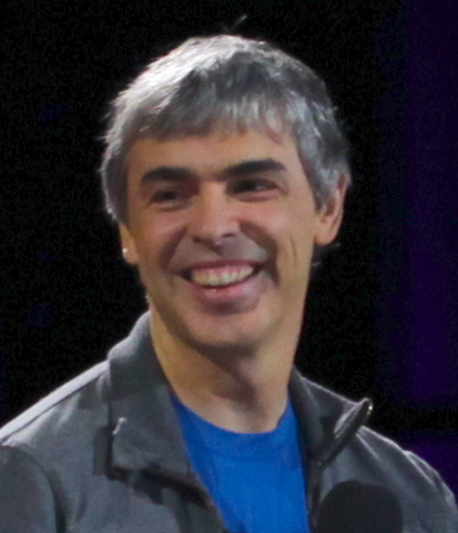
\includegraphics[width=\linewidth]{larry-page.jpg}\\
      {\scriptsize\color{gray}En 2014. Photo : Steve Jurvetson,
      CC BY 2.0, Wikimedia Commons.}
    \end{column}
    \begin{column}{0.72\textwidth}
      \begin{itemize}
        \item Né à East Lansing (Michigan) ; ses deux parents enseignent
          l'informatique. Doctorat à Stanford en 1995 (Terry Winograd) ;
          il y rencontre Sergey Brin.
        \item Analogie avec les citations : un article souvent cité, surtout
          par des articles importants, est important. Le robot du projet
          BackRub télécharge les liens du Web dès 1996.
        \item « The PageRank Citation Ranking » (1999) ; jeu de mots entre
          son nom et la page web. Brevet de Stanford, licence exclusive à
          Google.
        \item Septembre 1998 : Google, dans un garage de Menlo Park ; il
          abandonne son doctorat. PDG jusqu'en 2001, puis de 2011 à 2015 ;
          Alphabet jusqu'en 2019.
      \end{itemize}
    \end{column}
  \end{columns}
\end{frame}

% ═══════════════════════════════════════════════════════════════════════
\section{Synthèse}
% ═══════════════════════════════════════════════════════════════════════

\begin{frame}{Ce qu'il faut retenir}
  \small
  \begin{itemize}
    \item Probabilités totales : « multiplier le long d'une branche,
      additionner les branches » --- une ligne d'un produit matriciel.
    \item Chaîne de Markov : l'avenir ne dépend que du présent ; la loi
      évolue par $\vec x_{n+1}=M\vec x_n$, avec $M$ stochastique (colonnes
      de somme $1$).
    \item L'équilibre $\vec q=M\vec q$ : un vecteur propre de valeur
      propre $1$, et un point fixe ; limite des probabilités et proportion
      du temps passé dans chaque état.
    \item Si $M$ est régulière : un unique équilibre, atteint depuis
      n'importe quel départ ; la vitesse dépend de $|\lambda_2|$.
    \item PageRank : corriger les pages sans lien ($B$), puis téléporter
      ($G=\beta B+(1-\beta)U$).
    \item Méthode des puissances : $G$ est une contraction de rapport
      $\beta$ pour $d_1$ ; Banach garantit la convergence et borne
      l'erreur.
  \end{itemize}
\end{frame}

\begin{frame}{Un même point fixe, trois chapitres}
  \small
  \begin{center}
  \begin{tabular}{lll}
    \toprule
    Chapitre & Espace complet & Point fixe \\
    \midrule
    2 & $I\subset\R$ fermé & le zéro cherché par Newton \\
    3 & $\big(\Comp{\R^2},\dH\big)$ & une fractale \\
    4 & $(\Delta,d_1)$ & le PageRank du Web \\
    \bottomrule
  \end{tabular}
  \end{center}
  \vspace{6pt}
  À l'origine de l'une des plus grandes entreprises du monde : un projet
  de doctorat dont le cœur est le calcul d'un vecteur propre associé à la
  valeur propre $1$.
\end{frame}

\begin{frame}{Et maintenant}
  \begin{itemize}
    \item Les démonstrations laissées « au tableau » aujourd'hui sont
      toutes dans les notes de cours, avec tous les détails.
    \item Les exercices du chapitre (avec solutions complètes) couvrent
      chacun des résultats vus : à travailler avant le prochain cours.
    \item Les programmes Python des notes (météo, simulation, mini-webs,
      méthode des puissances) sont à exécuter et à modifier.
    \item Les rappels d'algèbre linéaire (valeurs propres,
      diagonalisation) sont à l'annexe D.
  \end{itemize}
\end{frame}


\end{document}
